\chapter{\;\;\;\;Verification Techniques}
\label{sec:overview-verification}

\section{Background}
\label{sec:overview-verification:background}

\section{Problems}
\label{sec:overview-verification:problems}
%% \myparagraph{Problems}
%
%   9051 /   2839 = 3.2 (id)
%  22124 /   8129 = 2.7 (ext)
%  23564 /   9128 = 2.6 (inj)
%
% Total
%  54739 /  20096 = 2.7  (pass)
% 152363 /  92029 = 1.65 (meta)
% 207102 / 112125 = 1.84 (whole)
%
%% Structured simulations of \ccc{} suffer from the problem that
%% verification using them is significantly more costly than that using
%% closed simulations of \cc{}: the Coq scripts for the verification of
%% all passes in \ccc{} is roughly \todo{2.7} times as large as that in
%% the original \cc{} in terms of lines of code~(LOC).
%% \jeehoon{How about reporting significant lines of code (SLOC)?}


%\section{Refinement Under Self-related Contexts (RUSC)}
\section{Our Solution}
\label{sec:overview-verification:solution}

%% \myparagraph{Our Solution at High Level}
%

% BEGIN REVISION
{\revisioncmd
\section{Memory Relations of \ccm{}}
\label{sec:overview-verification:injection}

\ccm{} uses the original memory identity and extension of \cc{}
(\Cref{sec:overview-verification:injection:original}) and mildly
strengthens the original memory injection to reason about dynamically allocated
local memory such as a function's stack frame for \emph{open} modules,
which can be compared to the structured injection of \ccc{}
(\Cref{sec:overview-verification:injection:dynamic}).
Moreover, we generalize it further to reason about statically allocated local memory
such as static variables of C by allowing module-local invariants on those static variables
(\Cref{sec:overview-verification:injection:static}).

%% and mildly generalize the memory injection of \cc{} in two steps: first to reason
%% about dynamic local memory such as a function's stack frame
%% (\Cref{sec:overview-verification:injection:dynamic}) and further to
%% reason about static local memory such as static variables of C
%% (\Cref{sec:overview-verification:injection:static}).
%% Structured injections of \ccc{} can be compared to our first generalization

\subsection{Memory Relations of \cc{}}
\label{sec:overview-verification:injection:original}
%
\cc{}'s memory model consists of a finite set of blocks of finite size
and a pointer value (or, an address) is a pair $(b,o)$ of a block id $b$ and an offset $o$ inside it.
The memory identity imposes that the source and target memories are identical;
and the extension that the two memories contain identical block ids and
each target block extends the corresponding source block
with more space and any values in it at the end.

A memory injection injects a subset of the source blocks into target blocks
without overlap. More precisely, a (selected) whole source block is injected into a single target block
while allowing multiple source blocks to be injected into the same target block without overlap.
This injection map specifies the \emph{public} areas of the source and target memories and the correspondence between them.
In other words, the corresponding addresses by the injection map are treated as \emph{equivalent} (public) pointer values,
%% and therefore
so that at those corresponding addresses,
only equivalent%
\footnote{Technically speaking, \cc{} allow more undefined values in the source
  because it proves refinement rather than equivalence between the source and target programs.}
values (\ie equivalent non-pointer values or corresponding addresses) should be stored .
All the areas that are not on the injection map are considered as \emph{private} areas of the source and target memories.

\subsection{Enriched Memory Injection}
\label{sec:overview-verification:injection:dynamic}
%
For open modules, reasoning about dynamically allocated local memory
such as a function's stack frame requires to strengthen the original
memory injection due to the presence of unknown modules.  The reason
is because when reasoning about a module $M$, we have to assume that
an unknown function invoked by $M$ does not change the dynamic local
memory of $M$ and also guarantee that a function of $M$ invoked by an
unknown module does not change the caller's dynamic local memory.

For this purpose, \ccc{} introduces \emph{structured injections} that
enrich the original memory injections with ownership information (\ie
whether owned by the current module or others) for all memory blocks
including public ones.  Using them, structured simulations impose
fine-grained invariants subject to the ownership information and a
concrete leakage protocol based on reachability from pointers.

Unlike \ccc{}, \ccm{} generalizes open simulations and memory injections
in a more abstract way following \cite{DBLP:conf/icfp/DreyerNB10,pb}.

First, we generalize the external call case of the open simulation in \Cref{fig:open-sim}
by allowing \emph{private transitions}, denoted $\sqsupseteq_\weak$,
as follows (\textcolor{red}{in red color}):
\[
\begin{array}{@{}l@{}}
\texttt{ 5:}~\quad \textcolor{red}{\exists w' \sqsupseteq_\weak w},~ (f_\src,f_\tgt)\in \texttt{vrel}(\textcolor{red}{w'}) \land (\vec{v}_\src,\vec{v}_\tgt) \in \overrightarrow{\texttt{vrel}(\textcolor{red}{w'})} \land{} \\[1mm]
\texttt{ 6:}~\quad \textcolor{red}{\forall w'' \sqsupseteq w'},~\forall (\memsrc',\memtgt')\in\texttt{mrel}(\textcolor{red}{w''}),~ \forall (r_\src,r_\tgt)\in \texttt{vrel}(\textcolor{red}{w''}),\\[1mm]
\texttt{ 7:}~\quad \textcolor{red}{\exists w''' \sqsupseteq_\weak w'',~ w''' \sqsupseteq w} \land {} \\
\phantom{\texttt{ 7:}}~\quad ((\memsrc',\mathtt{after\_external}~r_\src~\stsrc),(\memtgt',\mathtt{after\_external}~r_\tgt~\sttgt))\in R(\textcolor{red}{w'''})
\end{array}
\]
Though private transitions are allowed before and after an external function call (\ie
$w' \sqsupseteq_\weak w$ and $w''' \sqsupseteq_\weak w''$),
the overall transition should be \emph{public} (\ie $w''' \sqsupseteq w$)
assuming the external call also makes a public transition (\ie $w'' \sqsupseteq w'$).%
\footnote{We only allow private transitions just before and after external calls for simplicity.
See \Cref{sec:related} for comparison with \cite{DBLP:conf/icfp/DreyerNB10,pb}.}

Second, we extend memory injections to specify others' dynamic local
memories in the source and target that should be unchanged by the current module.
Specifically, an (enriched) memory injection $(\iota, m^\weak_\src, m^\weak_\tgt)$
consists of an original memory injection $\iota$ mapping the source public blocks into target blocks; and additionally
a private (\ie dynamic local) memory of the source $m^\weak_\src$ and that of the target $m^\weak_\tgt$
where $m^\weak_\src$ and $m^\weak_\tgt$ should be disjoint from the public memories specified by~$\iota$.
Then, private transitions from $(\iota, m^\weak_\src, m^\weak_\tgt)$ to
$(\iota', {m'}^\weak_\src, {m'}^\weak_\tgt)$ only require that $\iota'$ should extend $\iota$,
while public transitions additionally require that private memories should be unchanged
(\ie $m^\weak_\src = {m'}^\weak_\src$ and $m^\weak_\tgt = {m'}^\weak_\tgt$).
Note that all the areas of the source and target memories that are not on $m^\weak_\src$, $m^\weak_\tgt$ or the injection map $\iota$
are considered as \emph{private} (\ie dynamic local) memory of the current module.

\begin{wrapfigure}{r}{0.45\textwidth}
\begin{minipage}{0.45\textwidth}
\mbox{}\\[-7mm]    
\begin{Verbatim}
   int f() {          int f() {     
1:   int a0;            int a[2];   
2:   reg a1 = 0;  -->   a[1] = 0;   
3:   g(&a0);            g(&a[0]);   
4:   return a1;         return a[1];
   }                  }
\end{Verbatim}
\mbox{}\\[-10mm]
\end{minipage}
\end{wrapfigure}
To show how it works,
we give an example mimicking register spilling
in the presence of address-taken stack variables.
Consider the transformation on the right, where
in the source a memory block for \texttt{a0} and a function-local register for \texttt{a1} are allocated and
the address of \texttt{a0} escapes to \texttt{g},
while in the target a single block for both \texttt{a[0]} and \texttt{a[1]}
is allocated and the address of the block escapes to \texttt{g}.
Here \texttt{a0} can be seen as an address-taken stack variable and \texttt{a1} a spilled register.
The key difference is that, in the source, \texttt{a1} cannot be accessed by
\texttt{g} since it is a function-local register
while, in the target, \texttt{a[1]} can be accessed via the address of \texttt{a[0]}.

We now show how the target \texttt{f} simulates the source \texttt{f}
by logically protecting \texttt{a[1]} from \texttt{g}.
Though we give an informal description here to help understanding,
the formal definition of an open simulation $R$ 
can be easily derived from the description.
At line~$\texttt{1}$, any world $w_0$ and
memories $(m_\src, m_\tgt)$ related at $w_0$ are given. We take a step
to line~$\texttt{2}$ by extending $w_0.\iota$ (\ie the public
injection of $w_0$) to map $\texttt{a0}$ to $\texttt{a[0]}$, say $w_1$,
which is a public transition. At line~$\texttt{2}$, we take a step
to line~$\texttt{3}$ without changing the world $w_1$.
At line~$\texttt{3}$, we first make a private transition from $w_1$
to $w_2$ by extending $w_1.m^\weak_\tgt$
%(\ie the private area of the target memory)
to include the memory chunk $\texttt{a[1]} = 0$.
Then we assume that \texttt{g} makes a public transition from $w_2$ to $w_3$
returning any memories related at $w_3$. Thanks to $w_2.m^\weak_\tgt = w_3.m^\weak_\tgt$,
we know that the chunk $\texttt{a[1]} = 0$ remains the same.
Then we make a private transition from $w_3$ to $w_4$ by
dropping the chunk $\texttt{a[1]} = 0$ from $w_3.m^\weak_\tgt$.
Since $w_4.m^\weak_\tgt = w_1.m^\weak_\tgt$, we have a public transition from $w_1$ to $w_4$.
Finally, at line~$\texttt{4}$, we know that both the register $\texttt{a1}$ and
the memory-allocated variable $\texttt{a[1]}$ contain
$\texttt{0}$ and thus the same value $\texttt{0}$ is returned.

It is important to note that the (others') private memories $w.m^\weak_\src$ and $w.m^\weak_\tgt$ of a
memory injection $w$ are preserved as long as a function accesses
$(i)$ the memory via public addresses, or $(ii)$ its own private memory.
In the former case,
since a public block of the source is fully injected into a block of the target,
%% ---this is why the mapping is called an injection---
whenever a pointer offset goes beyond the public area mapped by the injection $w.\iota$,
the source program accesses an unallocated area thereby raising UB.
In the example above, if \texttt{g} in the target accesses \texttt{*(\&a[0]+1)},
then in the source it accesses \texttt{*(\&a0+1)}, which raises UB.
In the latter case, since the function's own private memory
is disjoint from all the memories specified by~$w$,
accessing it does not affect $w$. In the example above, at line~\texttt{2} in the target, 
the assignment \texttt{a[1] = 0} preserves $w_1.m^\weak_\tgt$ (and also the target public memory of $w_1$) because we know that
the current private memory \texttt{a[1]} is disjoint from the area specified by $w_1$ by construction.

\newrevision{Also note that any part of the public memories cannot be
  converted to a private one since the injection map is only
  extended at each step; and any part of the others' private memories
  (\ie $m^\weak_\src$ and $m^\weak_\tgt$) cannot be
  converted to the current module's private one since all
  \emph{proper} steps (\ie local steps or steps across an external
  call) only allow public transitions (\ie preserving $m^\weak_\src$ and $m^\weak_\tgt$).}

%% $R(w)$ relates any memories related at $w$ and
%% we take a step to line~$\texttt{2}$ by extending $w.\iota$
%% (\ie the (public) injection of $w$)
%% to map $\texttt{a0}$ to $\texttt{a[0]}$. At line~$\texttt{2}$,
%% $R(w)$ requires that $w.\iota$ maps $\texttt{a0}$ to $\texttt{a[0]}$

%% We now show how to logically protect \texttt{a[1]} from \texttt{g} and
%% prove that the two programs are related by an open simulation $R$.
%% First, $R$ relates each corresponding line of \texttt{f} in the source
%% and target.  We will then explain, at each line, how $R$ relates
%% source and target memories and satisfies the open simulation property.
%% At line~$\texttt{1}$, $R(w)$ relates any memories related at $w$ and
%% we take a step to line~$\texttt{2}$ by extending $w.\iota$
%% (\ie the (public) injection of $w$)
%% to map $\texttt{a0}$ to $\texttt{a[0]}$. At line~$\texttt{2}$,
%% $R(w)$ requires that $w.\iota$ maps $\texttt{a0}$ to $\texttt{a[0]}$

%% First,
%% we define an open simulation $R(w)$ to relate any memories related at
%% $w$ and each corresponding line of \texttt{f} in the source and
%% target. Second, we prove that 

%% Explain open simulation

\subsection{Memory Injection with Module-Local Invariants}
\label{sec:overview-verification:injection:static}
%
For open modules, reasoning about statically allocated local memory
such as static variables of C requires a further generalization.  The
problem is that when an open module $M$ invokes an unknown function
$f$, one cannot assume that the static memory of $M$ is unchanged
during the call because $f$ may call back a function from $M$, which
may change the static memory. However, since the static memory is only
accessible to the known functions in $M$, one can find a certain
invariant on the static memory by analyzing all the functions of $M$
and expect that an external call preserves the invariant although the
static memory can be changed. Enabling such reasoning is simple:
\ccm{} just adds another component in a memory injection $w$ that
globally imposes a given invariant on selected static variables
disjoint from $w.m^\weak_\src$, $w.m^\weak_\tgt$ and $w.\iota$.
We give examples using module-local invariants in \Cref{sec:overview-modulelocal}.
} %%% END REVISION

\section{Mixed Simulation}
\label{sec:overview-verification:mixedsim}

While the target language of \cc{} is deterministic (more precisely,
the source is receptive and the target is determinate) thereby mostly
using forward simulations, the repaired interaction semantics of
\ccm{} is inherently nondeterministic to handle illegal interference from assembly modules
%% enforce the assembly calling conventions
(see \Cref{sec:overview-semantics}) thus preventing the
use of forward simulation.
%% While it is theoretically possible to convert the \cc{}
%% verification from forward to backward simulations, it would incur a
%% significant cost since a compiler pass typically compiles a single
%% instruction in the source down to several instructions in the target.
%% %% due to the nature of source and target languages and the size of verification.
%% For this reason, determinism
%% has been considered ``instrumental for the simulation proofs of the compiler passes and its absence
%% is a show stopper''~\cite{besson:intptr}.
% Extending \cc{}'s semantics with such nondeterministic features can potentially cause significant
% overhead, as it invalidates forward simulation and enforces one to use backward simulation, which
% effectively means one should re-establish simulation proof from the scratch.  In literature, it is
% even said that

In order to recover the ability to use forward simulation in the occasional presence of nondeterminism,
we adopt the idea of \emph{mixed (forward-backward) simulation} from \cite{neis:pilsner}.
%% To embrace nondeterminism with low verification cost, we develop more general simulations, called
%% \emph{mixed simulations}, that (mostly) allow forward reasoning in the (occasional) presence of
%% nondeterminism.
The key observation is that
the requirement for using forward simulations (\ie determinism of the target) is a per-state property,
not a per-language property: as long as a particular target machine state is \emph{locally deterministic} (\ie its next state is unique),
one can do forward simulation at that state.
%% conversion from backward to forward simulations
%% requires only the current target \emph{machine state}, not the entire target \emph{language}, to be
%% deterministic.
Based on this observation, mixed simulations selectively allow forward
simulation when the target is locally deterministic, in addition to
the default backward simulation.
%% for each pair of related machine states, we allow the verifier to
%% \emph{choose} to perform either forward or backward reasoning, requiring that forward reasoning is
%% used only for locally deterministic target machine states.
%
Specifically, we say that a relation $R$ is a (closed) mixed simulation if
for all $(\mssrc, \mstgt) \in R$,
\begin{enumerate}
\item
  $\forall e, \mstgt',~ \mstgt \estep{e} \mstgt' \implies {}
  \exists \mssrc',~ \mssrc \estep{\tau}^{\raisebox{-1mm}{\scriptsize$\ast$}} \estep{e}\estep{\tau}^{\raisebox{-1mm}{\scriptsize$\ast$}} \mssrc' \land (\mssrc', \mstgt') \in R$; or
\item
  $\forall e, \mssrc',~ \mssrc \estep{e} \mssrc' \implies {}
  \exists \mstgt',~ \mstgt \eustep{\tau}^{\raisebox{-1mm}{\scriptsize$\ast$}} \eustep{e}\eustep{\tau}^{\raisebox{-1mm}{\scriptsize$\ast$}} \mstgt' \land (\mssrc', \mstgt') \in R$\\
  where $\ms \eustep{e} \ms'$ denotes that $\ms$ is locally deterministic and $\ms \estep{e} \ms'$.
\end{enumerate}

\Cref{fig:mixedsim} visualizes this formulation of mixed simulation, where
%% presents an example of mixed simulations, where $R$ is a simulation relation; red and blue circle represent source and
%% target machine states, respectively;
solid and dotted arrows represent universally and existentially
quantified steps, respectively, and double circles represent locally
deterministic target states. In this figure,
since the first three target machine states are deterministic,
we can do forward simulation as shown in the figure;
then, since the following target state is nondeterministic,
we should do backward simulation as shown in the figure.
%% the first three target machine states are deterministic.  The
%% first three target steps are deterministic and reasoned in a forward manner (from source to target),
%% and the last target step is nondeterministic and reasoned in a backward manner (from target to
%% source).  Later, those part of simulations that are reasoned in a forward manner is converted to
%% backward reasoning, thereby proving backward simulation and thus behavior refinement.

Note that the repaired interaction semantics is nondeterministic only
at the initial step of a module invocation, so that we can do
forward simulation everywhere else using mixed simulations.

In order to support \cc{}'s condition for forward simulation,
we also add the following to the above formulation of mixed simulation:
\begin{enumerate}[resume]
\item or, $\mssrc$ is receptive and\\
  $\forall e, \mssrc',~ \mssrc \estep{e} \mssrc' \implies {}
  \exists \mstgt',~ \mstgt \exstep{\tau}^{\raisebox{-1mm}{\scriptsize$\ast$}} \exstep{e}\exstep{\tau}^{\raisebox{-1mm}{\scriptsize$\ast$}} \mstgt' \land (\mssrc', \mstgt') \in R$\\
  where $\ms \exstep{e} \ms'$ denotes that $\ms$ is locally determinate and $\ms \estep{e} \ms'$.
\end{enumerate}
Also we apply this mechanism of mixed simulation to our open simulations.

\begin{figure}[t]%% {0.43\textwidth}
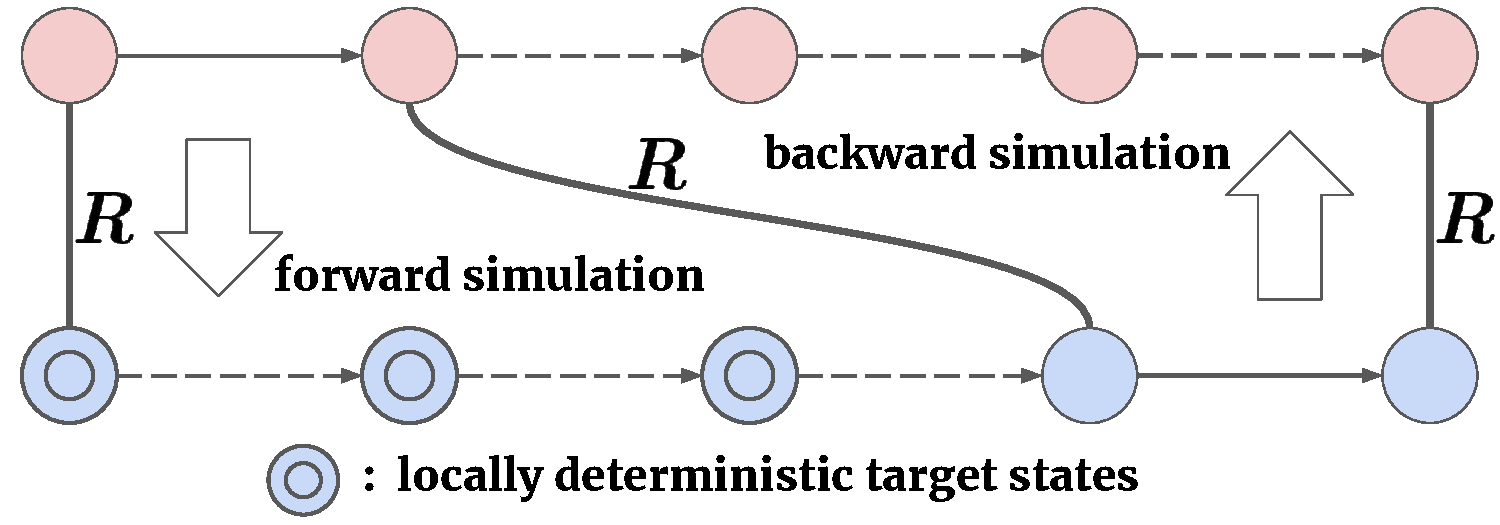
\includegraphics[width=0.7\textwidth]{images/mixed-sim-bold.pdf}
%% 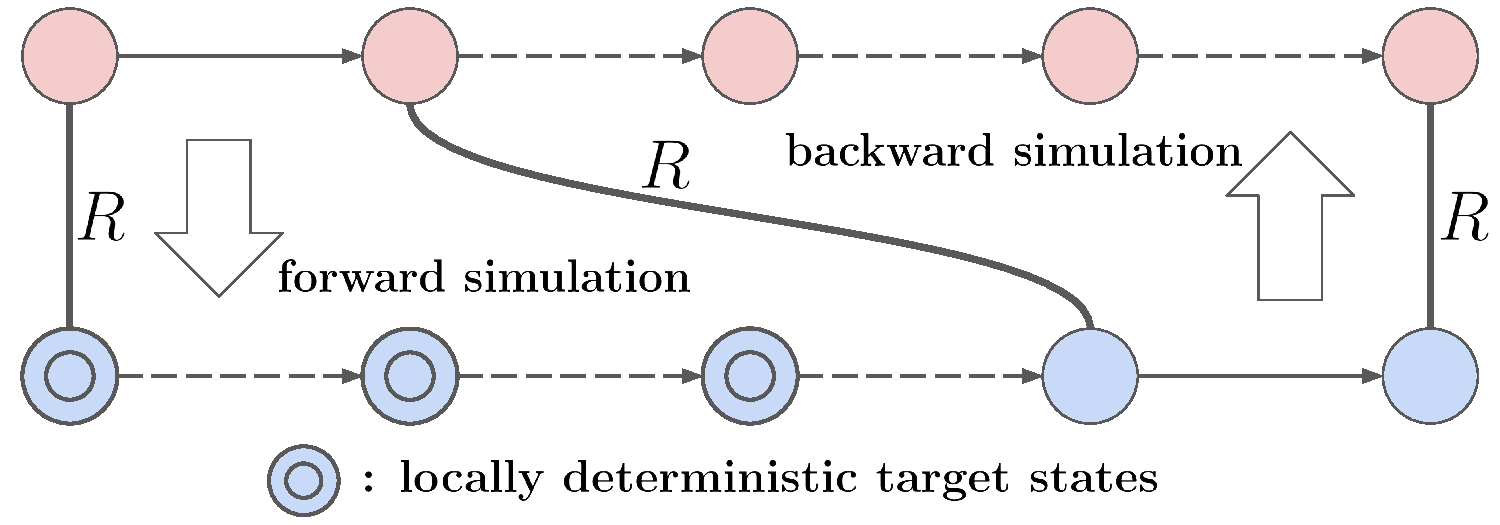
\includegraphics[width=0.7\textwidth]{images/mixed-sim.pdf}
\caption{A visualized example of mixed simulations}
\label{fig:mixedsim}
\end{figure}

%% Using mixed simulation, we verify the compositional correctness of \cc{} optimizations by
%% performing forward reasoning on deterministic target states, thereby reusing all the simulation proofs in \cc{}
%% and performing backward reasoning on nondeterministic target states which we
%% introduce in \ccm{}.
%% Furthermore, using mixed simulation, we can reduce the trusted computing base
%% of the original \cc{} by removing the assumption that external function calls are deterministic.
%% Mixed simulation is the first embodiment of the idea of exploiting determinism at the granularity of
%% machine states in the context of \cc{}, while the idea itself is first presented in
%% \cite{neis:pilsner}.

%% Specifically, \cc{}'s forward simulation actually requires a notion slightly different from
%% determinism (namely, that the source language is \emph{receptive} and the target language is
%% \emph{determinate}).  Our formalization supports both \cc{}-style forward simulation and the
%% Pilsner's one.

%%% Local Variables:
%%% mode: latex
%%% TeX-master: "main"
%%% End:
